\documentclass[12pt, fullpage,letterpaper]{article}
\usepackage[margin=1in]{geometry}
\usepackage{graphicx}
\title{CS6630 Visualization Fall 2017 Project \\ A Mirror of History}
\author{Yanqing Peng, Yuwei Wang}
\begin{document}
\maketitle
\newpage
\paragraph{Get started!} (Nov 4)

After spending a lot of time on data collecting, we successfully collected
the raw data of the historical country borders. The data we collected come
from two different data sets:

\begin{itemize}
    \item For maps after World War II (1946-2017), we collect from www.thenmap.net.
        Although this website doesn't provide the off-the-shelf dataset, one of its
        API support querying for the world map at a specific year after WW2. The API
        we used looks like following:

        \begin{verbatim}
        wget http://api.thenmap.net/v1/world-2/geo|data/1946?data_props=name|wikidata
        \end{verbatim}

        This query retrieves the world map at 1946 with the metadata of country name as well as
        the wikidata id for the country. The wikidata ID is essential for future data collection
        such as population.

    \item For maps from 2000BC to 1945, we find the dataset in a cartography forum (http://www.cartotalk.com/index.php?showtopic=3462).
        The author is anonymous.
        The dataset only contains a few years. That's reasonable enouth -- we never expect to
        find a dataset contains all data from 2000BC to 2017AD!

\end{itemize}

For other data (e.g. population), it seems promising to retrieve data from Wikidata.
We plan to explore the possibility for that.
The first dataset already include the Wikidata ID for all countries.
We may have to do some data processing on the second dataset to add the Wikidata ID information to it.

\newpage
\paragraph{Implementing the map} (Nov 5)

We implemented a prototype of the map chart and the year chart.
It looks like the follwing (Figure \ref{fig:nov5}):

\begin{figure}[h!]
    \begin{center}
        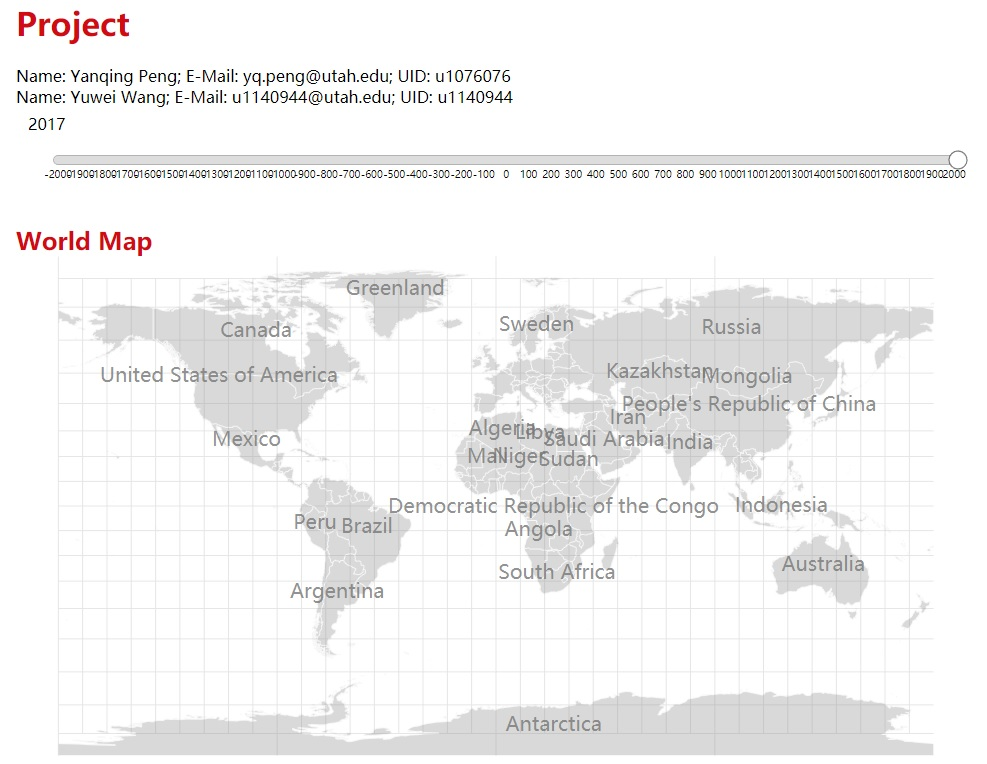
\includegraphics[width=0.7\textwidth]{figs/Nov5.jpg}
        \caption{Current state of our project, Nov 5.}
        \label{fig:nov5}
    \end{center}
\end{figure}

For the year chart, there is a slide bar and a circle which we can drag to choose the desired year.
When the choice of year is updated, the map chart read the dataset with the nearest year before the selected year,
and draw it on the screen. The projection we currently use is d3.geoPatterson().

Adding label is quite challenging. If we simply put all labels on the map,
then there will be a mess in Europe. Currently we only show the labels for countries
with area larger than a threshold. That doesn't work for countries with large area and extremely
long names (e.g. Democratic Republic of the Congo). Whether or not a label is shown
should depend on both country area and the length of country name. We should think carefully about it.

The location of the labels is another issue. Currently we put the label
at the centroid of the corresponding path. But it doesn't work for some countries like the U.S.
The label of U.S. is actually located inside Canada. We think it's because of Alaska.
We have to find a smarter way to locate the labels.

\newpage
\paragraph{Layout design, and more on label placement} (Nov 6)

We finished a prototype of the info panel. We also improved the label placement.
As shown in Figure \ref{fig:nov6}, now it looks better, isn't it?

\begin{figure}[h!]
    \begin{center}
        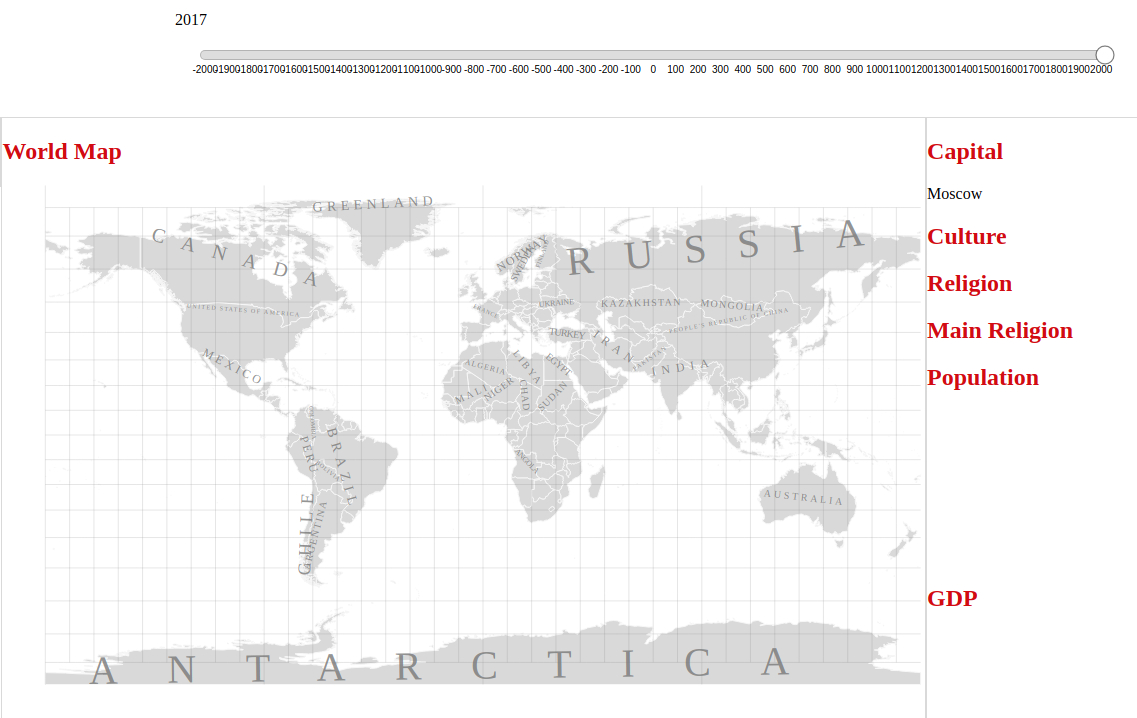
\includegraphics[width=0.7\textwidth]{figs/Nov6.png}
        \caption{Current state of our project, Nov 6.}
        \label{fig:nov5}
    \end{center}
\end{figure}

\end{document}
